% A book summary template inspired by Jan Küster's Left Sidebar CV / https://github.com/jankapunkt/latexcv

\documentclass[11pt,a4paper]{article}	
\usepackage[utf8]{inputenc}
\usepackage[authoryear]{natbib}
\usepackage{bibentry}
\usepackage{progressbar}
\usepackage{usebib}
% \newbibfield{booktitle}
% \bibinput{bibliography}


\usepackage[default]{raleway}

% set font default
\renewcommand*\familydefault{\sfdefault} 	
\usepackage[T1]{fontenc}

\usepackage{moresize}
\usepackage{fontawesome}
\usepackage{float}

\usepackage{paracol}
\usepackage[margin=1.5cm]{geometry}

\usepackage{fancyhdr}
\pagestyle{empty}
\setlength{\parindent}{0mm}
\usepackage{graphicx}
	
\usepackage{tikz}				
\usetikzlibrary{shapes, backgrounds,mindmap, trees}

\usepackage{transparent}
\usepackage{color}

\usepackage{ifthen}
\usepackage{calc}
\usepackage{pifont}
\usepackage{forloop}

\newcounter{starnumber}
\newcommand{\stars}[1]{
  \forloop{starnumber}{1}{\value{starnumber} < 6}{
    \ifthenelse{#1 < \value{starnumber}}{\ding{73}}{\ding{72}}%
  }
}

%!TEX root = ./main.tex

\definecolor{courserablue}{RGB}{42, 115, 204}
\definecolor{swedenyellow}{RGB}{254, 205, 0}
\definecolor{napiergreen}{rgb}{0.16, 0.5, 0.0}
\definecolor{tomato}{rgb}{1.0, 0.39, 0.28}
\colorlet{greyedout}{black!20}
\definecolor{kthblue}{RGB}{25,84,166}
\definecolor{nipspurple}{RGB}{129, 89, 152}
\definecolor{tennis}{RGB}{220, 253, 80}
% \colorlet{bookcolor}{kthblue}
\colorlet{bookcolor}{kthblue}
% \newcommand{\coverColor}{goldenbrown}

% \newcommand{\coverColor}{ocre}
% \newcommand{\coverTitleColor}{white}
% \newcommand{\bookColor}{ocre}
% \newcommand{\bookColor}{ocre}
\newcommand{\coverTitleColor}{white}
\newcommand{\bookColor}{bookcolor}
\newcommand{\coverColor}{\bookColor}


% \definecolor{maincol}{RGB}{ 225, 0, 0 }
\definecolor{darkcol}{RGB}{ 70, 70, 70 }
\definecolor{lightcol}{RGB}{245,245,245}
\colorlet{maincol}{bookcolor}
% \colorlet{darkcol}{bookcolor}

\usepackage{enumitem}
\setitemize{label={\color{maincol}\faCheck}}

\usepackage[hidelinks]{hyperref}
% A book summary template inspired by Jan Küster's Left Sidebar CV / https://github.com/jankapunkt/latexcv
% The following are the elements taken from said template, albeit from heading onwards was modified and made simpler or added as entirely new elements.



% use to vertically center content
% credits to: http://tex.stackexchange.com/questions/7219/how-to-vertically-center-two-images-next-to-each-other
\newcommand{\vcenteredinclude}[1]{\begingroup
\setbox0=\hbox{\includegraphics{#1}}%
\parbox{\wd0}{\box0}\endgroup}

% use to vertically center content
% credits to: http://tex.stackexchange.com/questions/7219/how-to-vertically-center-two-images-next-to-each-other
\newcommand*{\vcenteredhbox}[1]{\begingroup
\setbox0=\hbox{#1}\parbox{\wd0}{\box0}\endgroup}

% icon shortcut
\newcommand{\icon}[3] { 							
	\makebox(#2, #2){\textcolor{maincol}{\csname fa#1\endcsname}}
}	

% icon with text shortcut
\newcommand{\icontext}[4]{ 						
	\vcenteredhbox{\icon{#1}{#2}{#3}}  \hspace{2pt}  \parbox{0.9\textwidth}{\textcolor{#4}{#3}}
}

% icon with website url
\newcommand{\iconhref}[5]{ 						
    \vcenteredhbox{\icon{#1}{#2}{#5}}  \hspace{2pt} \href{#4}{\textcolor{#5}{#3}}
}

% icon with email link
\newcommand{\iconemail}[5]{ 						
    \vcenteredhbox{\icon{#1}{#2}{#5}}  \hspace{2pt} \href{mailto:#4}{\textcolor{#5}{#3}}
}

%---------------------------------------------------------
% MODIFIED from Kuester's CV
%---------------------------------------------------------
% Renders a a CV section headline with a nice underline in main color.
% param 1: section title
\newcommand{\heading}[1] {
	\vspace{15pt}
	{\bf\LARGE\color{darkcol}\uppercase{#1}}\\[-4pt]
	{\color{maincol}\rule{0.1\textwidth}{2pt} }\vspace{2pt}
}

%---------------------------------------------------------
% New 
%----------------------------------------------------------
\newcommand{\titlebox}[3]
{\fcolorbox{#1}{#2}{\begin{minipage}[c][3.0cm][c]{\linewidth}%
\begin{center}\large\color{white} #3 %
\end{center}\end{minipage}\\[14pt]
\vspace{-12pt}
}
}

\newcommand{\bigfont}[1]{%
{\bf\large\uppercase{#1} } \\[4pt]%
\rule{0.1\textwidth}{1.25pt} \\[4pt]%
}

\newcommand{\titletext}[1]{%
#1 \\[4pt] %
\rule{0.1\textwidth}{1.25pt} \\[4pt]%
}

\renewenvironment{quote}
               {\list{\Large\color{black!50}\faQuoteLeft\phantom{ }}{\rightmargin\leftmargin}%
                \item\relax\Large\color{black!50}\ignorespaces}
               {\unskip\unskip\phantom{xx}\color{black!50}\faQuoteRight\normalsize\endlist}
           





%============================================================================%
\begin{document}
\columnratio{0.31}
\setlength{\columnsep}{2.2em}
\setlength{\columnseprule}{4pt}
\colseprulecolor{lightcol}
\begin{paracol}{2}


\heading{Overview}

\small


% \newcommand{\paperkey}{Gu2018}

\icontext{Male}{12}{Gu et al.}{black}\\[6pt]	
\icontext{Book}{12}{ICSE}{black}\\[6pt]	
% \icontext{MapMarker}{12}{NY}{black}\\[6pt]
\icontext{Calendar}{12}{2022}{black}\\[6pt]
\icontext{Github}{12}{\href{https://github.com/guxd/deep-code-search}{Source code}}{black}\\[6pt]
% \iconemail{Laptop}{12}{Book Website}{https://gregmckeown.com/book/}{black}\\[6pt]
% \iconemail{Globe}{12}{Summary Source 1}{https://epigrammetry.hypotheses.org/595}{black}\\[6pt]
% \iconemail{Globe}{12}{Summary Source 2}{https://epigrammetry.hypotheses.org/248}{black}\\[6pt]
\icontext{Database}{12}{GitHub (Java)}{black}\\[6pt]
\icontext{BarChart}{12}{Top-N (recall, precision, MRR,
F1)}{black}\\[6pt]
\icontext{Wrench}{12}{RNN, MLP, Fusion, Pooling}{black}\\[6pt]
\icontext{Bullseye}{12}{Code reuse, code search}{black}\\[6pt]
\icontext{QuoteRight}{12}{146}{black}\\[6pt]
% \icontext{Tachometer}{12}{\progressbar[filledcolor=bookcolor,emptycolor=bookcolor!20]{0.0}}{black}\\[6pt]
% \icontext{Star}{12}{\stars{5}}{black}\\[6pt]
\icontext{Star}{12}{\stars{5}}{black}\\[6pt]

\vspace{3em}

\normalsize
\switchcolumn

% \titlebox{white}{darkcol}{
\titlebox{white}{kthblue}{

{\bf\large Deep Code Search}  \\[4pt]
\rule{0.1\textwidth}{1.25pt} \\[4pt]

Gu et al. [2022]



}
\vspace{1em}



%---------------------------------------------------------------------------------------

\begin{figure}[H]
\begin{center}
    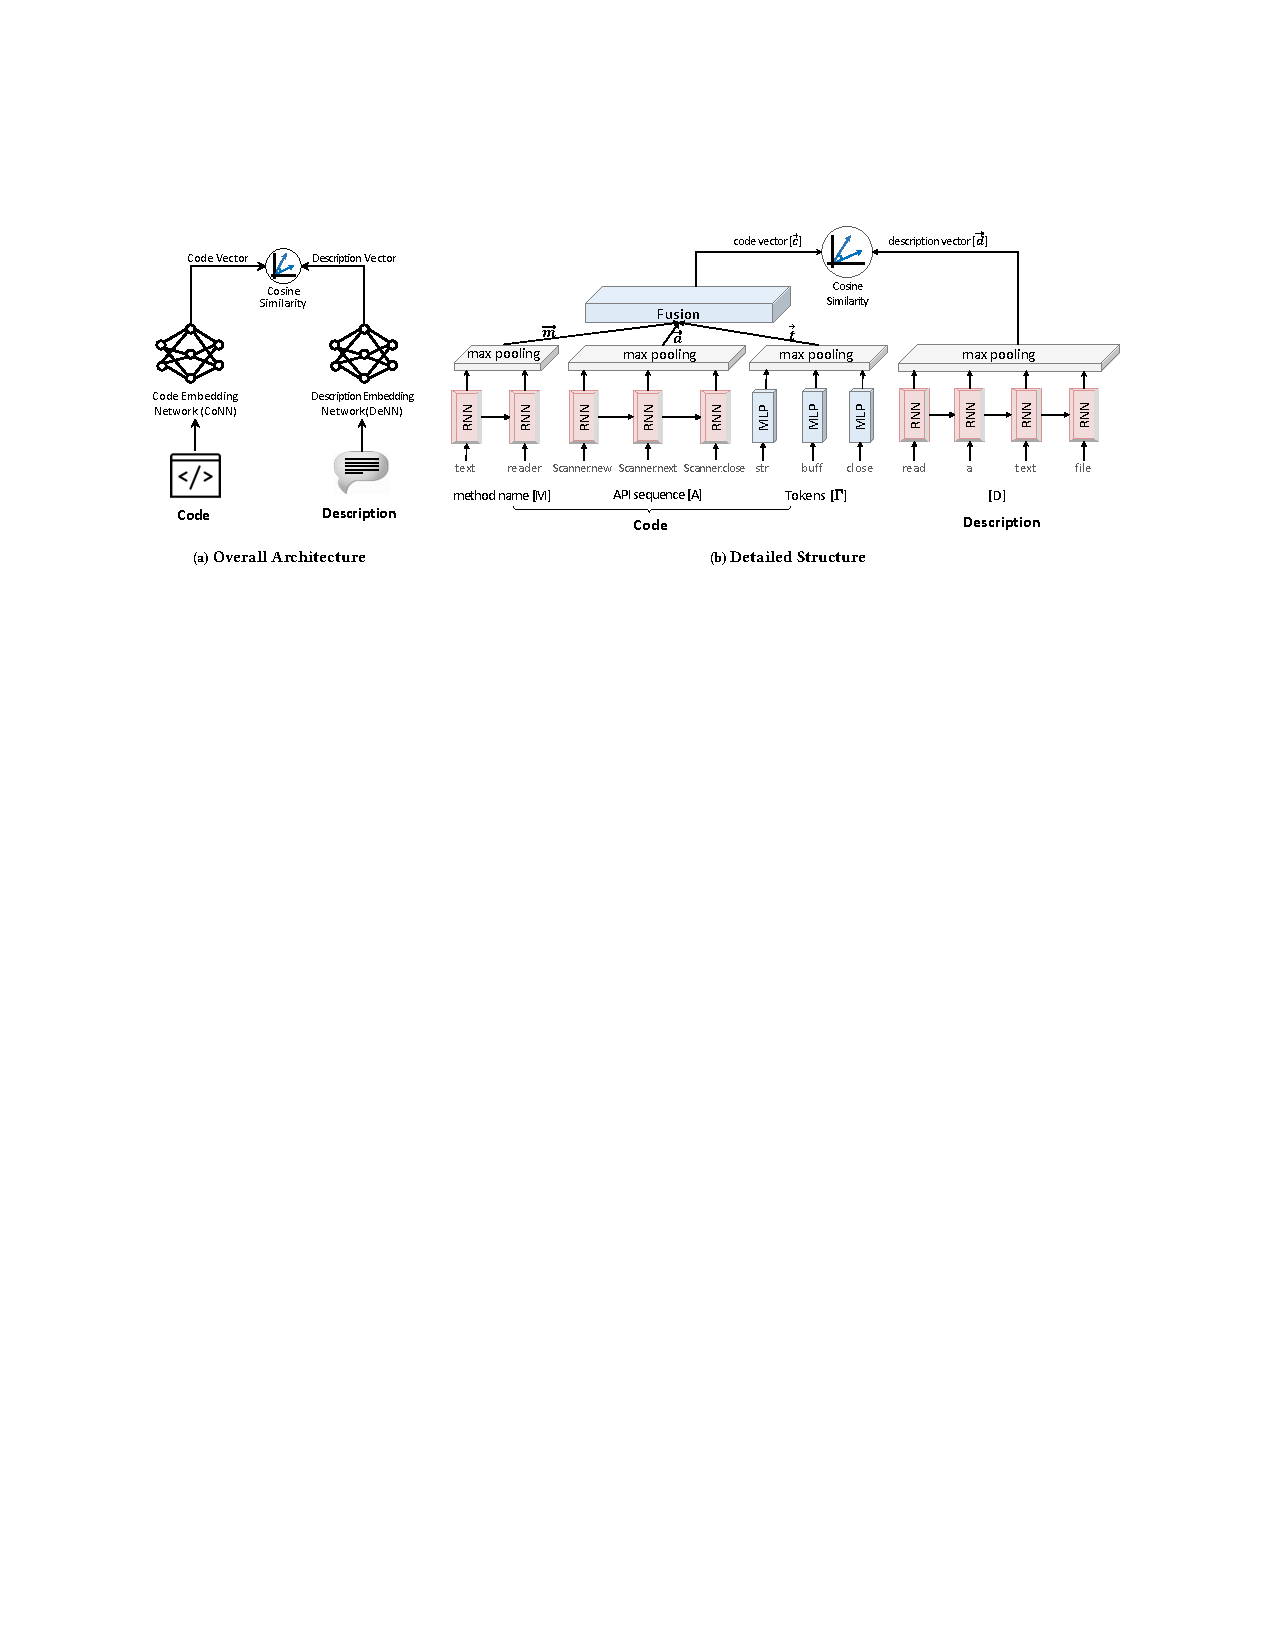
\includegraphics[width=\linewidth]{Gu2018-image.pdf}
\end{center}
\end{figure}

\heading{What did authors try to accomplish?}
\begin{itemize}
            \item Improve code search done with nautal language.
    \end{itemize}

\heading{Key elements}
\begin{itemize}
            \item Embedding code documentation and source code
embeddings into the same representation. In other words, the source code
embedding and its corresponding documentation embedding will have
similar vectors.
            \item A unified representation of heterogeneous data.
            \item Reinforcer-transformer architecture.
            \item Better query understanding through deep learning.
            \item Clustering snippets by natural language semantics.
    \end{itemize}

\heading{What can you use yourself?}
\begin{itemize}
            \item Embedding documentation and source code into the same
space is a powerful idea.
    \end{itemize}

\heading{Thoughts}
\begin{itemize}
            \item Depending on the application it can also be used for
our project.
    \end{itemize}

\heading{References to follow}

\begin{itemize}
            \item DeepAI.
    \end{itemize}


\end{paracol}
\end{document}
